\documentclass[12pt]{article}

\usepackage{amsmath, mathtools}
\usepackage{amsfonts}
\usepackage{amssymb}
\usepackage{graphicx}
\usepackage{colortbl}
\usepackage{xr}
\usepackage{hyperref}
\usepackage{longtable}
\usepackage{xfrac}
\usepackage{tabularx}
\usepackage{float}
\usepackage{siunitx}
\usepackage{booktabs}
\usepackage{caption}
\usepackage{pdflscape}
\usepackage{afterpage}
\usepackage[usenames,dvipsnames,table]{xcolor}
\usepackage{txfonts}

\usepackage[round]{natbib}

%\usepackage{refcheck}

\hypersetup{
    bookmarks=true,         % show bookmarks bar?
      colorlinks=true,       % false: boxed links; true: colored links
    linkcolor=Purple,          % color of internal links (change box color with 
    %linkbordercolor)
    citecolor=ForestGreen,        % color of links to bibliography
    filecolor=WildStrawberry,      % color of file links
    urlcolor=Cerulean           % color of external links
}

%% Comments

\usepackage{color}

\newif\ifcomments\commentstrue

\ifcomments
\newcommand{\authornote}[3]{\textcolor{#1}{[#3 ---#2]}}
\newcommand{\todo}[1]{\textcolor{red}{[TODO: #1]}}
\else
\newcommand{\authornote}[3]{}
\newcommand{\todo}[1]{}
\fi

\newcommand{\wss}[1]{\authornote{blue}{SS}{#1}}
\newcommand{\an}[1]{\authornote{magenta}{Author}{#1}}

% For easy change of table widths
\newcommand{\colZwidth}{1.0\textwidth}
\newcommand{\colAwidth}{0.13\textwidth}
\newcommand{\colBwidth}{0.82\textwidth}
\newcommand{\colCwidth}{0.1\textwidth}
\newcommand{\colDwidth}{0.05\textwidth}
\newcommand{\colEwidth}{0.8\textwidth}
\newcommand{\colFwidth}{0.17\textwidth}
\newcommand{\colGwidth}{0.5\textwidth}
\newcommand{\colHwidth}{0.28\textwidth}

% Used so that cross-references have a meaningful prefix
\newcounter{defnum} %Definition Number
\newcommand{\dthedefnum}{GD\thedefnum}
\newcommand{\dref}[1]{GD\ref{#1}}
\newcounter{datadefnum} %Datadefinition Number
\newcommand{\ddthedatadefnum}{DD\thedatadefnum}
\newcommand{\ddref}[1]{DD\ref{#1}}
\newcounter{theorynum} %Theory Number
\newcommand{\tthetheorynum}{T\thetheorynum}
\newcommand{\tref}[1]{T\ref{#1}}
\newcounter{tablenum} %Table Number
\newcommand{\tbthetablenum}{T\thetablenum}
\newcommand{\tbref}[1]{TB\ref{#1}}
\newcounter{assumpnum} %Assumption Number
\newcommand{\atheassumpnum}{P\theassumpnum}
\newcommand{\aref}[1]{A\ref{#1}}
\newcounter{goalnum} %Goal Number
\newcommand{\gthegoalnum}{P\thegoalnum}
\newcommand{\gsref}[1]{GS\ref{#1}}
\newcounter{instnum} %Instance Number
\newcommand{\itheinstnum}{IM\theinstnum}
\newcommand{\iref}[1]{IM\ref{#1}}
\newcounter{reqnum} %Requirement Number
\newcommand{\rthereqnum}{P\thereqnum}
\newcommand{\rref}[1]{R\ref{#1}}
\newcounter{lcnum} %Likely change number
\newcommand{\lthelcnum}{LC\thelcnum}
\newcommand{\lcref}[1]{LC\ref{#1}}

\newcommand{\progname}{Companion Cube Calculator} % PUT YOUR PROGRAM NAME HERE
\newcommand{\prognameAbbrv}{$C^{3}$}

\usepackage{fullpage}

\begin{document}

\title{Companion Cube Calculator} 
\author{Geneva Smith}
\date{\today}
	
\maketitle

~\newpage

\pagenumbering{roman}

\section{Revision History}

\begin{tabularx}{\textwidth}{p{3cm}p{2cm}X}
\toprule {\bf Date} & {\bf Version} & {\bf Notes}\\
\midrule
 & 1.0.2 & Collapsed theoretical models for addition, subtraction, and 
 multiplication into one model\\
October 18, 2017 & 1.0.1 & Revised table of units and documentation notations \\
October 4, 2017 & 1.0 & Completed the initial SRS documentation\\
\bottomrule
\end{tabularx}

~\newpage

\section{Reference Material}

This section records information for easy reference.

\subsection{Table of Units}

The tasks performed by the \prognameAbbrv{} tool are unitless.

\subsection{Table of Symbols}

The table that follows summarizes the symbols used in this document. The choice 
of symbols was made to be consistent with mathematical notations of functions, 
sets, and intervals. The symbols are listed in alphabetical order.

\renewcommand{\arraystretch}{1.2}
\noindent \begin{longtable*}{m{1.5cm} m{5.3cm} m{8.2cm}} \toprule
\textbf{Symbol}  & \textbf{Type} & \textbf{Description}\\
\midrule 
\endhead
$a$ & $\varmathbb{R}$ & The minimum bound in an interval\\
$b$ & $\varmathbb{R}$ & The maximum bound in an interval\\
$[a,b]$ & $[\varmathbb{R}, \varmathbb{R}]$ & Closed interval with endpoints $a$ 
and $b$\\
$(a,b)$ & $(\varmathbb{R}, \varmathbb{R})$ & Open interval with endpoints $a$ 
and $b$\\
$B$ & $\varmathbb{R}$ & Base number in exponentiation (e.g. $B^2$)\\
$D(v)$ & $[\varmathbb{R}, \varmathbb{R}]$ & The domain of a variable $v$ 
represented as a closed, real interval $x$\\
$f(x)$ & $Type$ & A mathematical function on a variable $x$; the 
function type is determined by the type of $x$\\
$f(V)$ & $\{[\varmathbb{R}, \varmathbb{R}]_0, ..., [\varmathbb{R}, 
\varmathbb{R}]_n\} \rightarrow [\varmathbb{R}, 
\varmathbb{R}]$ & A function of domains for a set of variables $V$ that 
produces a closed, real interval\\
$M$ & - & A temporary variable for aiding in the readability of equations\\
$\varmathbb{N}$ & - & The set of natural numbers; assumes that $0$ is included 
in this specification\\
$N$ & $\varmathbb{N}$ & Power in exponentiation (e.g. $2^N$) \\
$n$ & $\varmathbb{N}$ & A variable subscript denoting placement in an ordered 
set\\
$op$ & $Type \rightarrow Type \rightarrow Type$ & A temporary set of 
mathematical operators used to define equation templates; the type of the 
equation is determined by the type of the input values\\
$\varmathbb{R}$ & - & The set of real numbers\\
$R(f(V))$ & $[\varmathbb{R}, \varmathbb{R}]$ & The range of $f(V)$ represented 
as a closed, real interval\\
$V$ & - & A set of variable names\\
$v$ & - & A variable name\\
$X$ & $\{\varmathbb{R}_0, ..., \varmathbb{R}_n\}$ & A closed, connected set of 
real values\\
$x$ & $\varmathbb{R}$ & An element of $X$\\
$Y$ & $\{\varmathbb{R}_0, ..., \varmathbb{R}_n\}$ & A closed, connected set of 
real values\\
$y$ & $\varmathbb{R}$ & An element of $y$\\
$z$ & $\varmathbb{R}$ & A temporary value used in operations between $X$ and 
$Y$\\
\bottomrule
\end{longtable*}

\subsection{Abbreviations and Acronyms}

\renewcommand{\arraystretch}{1.2}
\begin{tabular}{l l} 
  \toprule		
  \textbf{Text} & \textbf{Description}\\
  \midrule 
  A & Assumption\\
  CRPG & Computer Role-Playing Game\\
  DD & Data Definition\\
  GD & General Definition\\
  GS & Goal Statement\\
  GUI & Graphical User Interface\\
  IM & Instance Model\\
  LC & Likely Change\\
  NPC & Non-Player Character (Games)\\
  PS & Physical System Description\\
  R & Requirement\\
  SRS & Software Requirements Specification\\
  \prognameAbbrv{} & \progname{}\\
  T & Theoretical Model\\
  \bottomrule
\end{tabular}

\newpage

\tableofcontents

~\newpage

\pagenumbering{arabic}

\section{Introduction}
\label{intro}
This document is an SRS for the \progname{} (\prognameAbbrv{}), a mathematical 
tool which determines the range, $R(f(V))$, of a user-specified function, 
$f(V)$, given the domains of the function's variables, $D(v), v \in V$. This 
tool will aid in the specification and refinement of GLaDOS, an emotion engine 
for Non-Player Characters (NPCs) in Computer Role-Playing Games (CRPGs) as 
described by \citet{glados}.

\subsection{Purpose of Document}
This document outlines the requirements identified for the development of the 
\prognameAbbrv{} tool, including the product goals, product scope, and the 
concrete mathematical models driving the design. It also describes the 
assumptions and theoretical models used to influence the concrete models. The 
purpose of documenting this information is to aid in future use, maintenance, 
and development of the \prognameAbbrv{} tool.

This document is intended for two reader types -- those who wish to use the 
tool and those who wish to refine and expand the tool. Even though the 
\progname{} was created specifically to aid in the development of the GLaDOS 
architecture, the user specified $f(V)$ is unitless. This means that the tool 
can be used for any $f(V)$ as long as any applicable units referred to in 
$D(v), v \in V$ are compatible.

Since the initial development of the \prognameAbbrv{} tool will be limited to 
arithmetic operators, this document includes information that is useful to a 
developer looking to expand the abilities of the \prognameAbbrv{} with 
additional mathematical models to suit their project, such as those proposed in 
\lcref{LC_trig} and \lcref{LC_infinity}. 

\subsection{Scope of Requirements} 
The \prognameAbbrv{} calculates $R(f(V))$ of a user-defined $f(V)$ and variable 
domains $D(v), v \in V$. Each $D(v)$ must be specified by the user in the 
initial version of this tool, otherwise the tool will assume that the user 
input set is incomplete and treat it as an error.

For the initial version of this product, the mathematical operations allowed in 
an function will be limited to brackets ($()$) and the set of mathematical 
operators $\{+, -, \times, \div, B^x, x^N\}$. Future iterations can expand this 
list to include trigonometric functions ($\sin(x)$, $\cos(x)$, $\tan(x)$, 
$\arcsin(x)$, $\arccos(x)$, $\arctan(x)$), partial functions, and other useful 
mathematical constructs.

Division is a special case in the \prognameAbbrv{} tool because of its 
behaviour around zero. Division by zero is an undefined term, but can be 
represented by the open interval $(-\infty, \infty)$. This version of the 
\prognameAbbrv{} tool can only process closed intervals (\aref{A_interval}), 
meaning that a divisor interval that contains zero cannot be handled correctly. 

The initial version of the tool is intended for use during the development of 
the GLaDOS architecture. The values calculated by the architecture are 
normalized, so any uncertainties in the bounds of $R(f(V))$ can be ignored in 
this context because it is assumed that any calculation errors will not have a 
noticeable affect on the architecture's processing. Therefore, directed 
rounding is not required for the initial version of the \prognameAbbrv{} tool.

The purpose of this product is to aid in the design and tuning of the GLaDOS 
architecture (Section~\ref{Sec_pd}), but it can be used in similar projects 
because it does not contain any GLaDOS-specific concepts or models.

\subsection{Characteristics of Intended Reader}
\label{intro_reader}
The intended reader of this document must understand elementary algebra, 
especially interval arithmetic, in the domain of real numbers 
($\varmathbb{R}$). An understanding of set notation is also required to 
understand the models presented in this document. They must also have an 
understanding of domain and range with respect to a function in order to 
understand the outputs of the product 
and how it relates to its inputs.

\subsection{Organization of Document}
This document begins by describing the general description of the 
\prognameAbbrv{} tool (Section \ref{general}), which includes the system 
context, constraints, and the intended users' characteristics. This is followed 
by a description of the problem to be solved, including the models and 
assumptions that are used to address it (Section \ref{specific}). This 
description is followed by the functional and non-functional requirements of 
the \prognameAbbrv{} tool (Section \ref{requirements}) and suggested 
refinements and expansions for future iterations (Section \ref{changes}). The 
last section in this document, traceability matrices and graphs (Section 
\ref{trace}), visually describes the dependencies between different document 
components. This information can be referenced when making changes to the 
tool's core specifications.

\section{General System Description}
\label{general}

This section identifies the interfaces between the system and its environment,
describes the user characteristics, and lists the system constraints.

\subsection{System Context}
The \prognameAbbrv{} tool is a stand-alone application for calculating 
$R(f(V))$ for a user-defined $f(V)$ given the known $D(v), v\in V$. Therefore 
it is independent and self-contained with respect to external organizations, 
products, and technologies.

The user interface of the \prognameAbbrv{} tool facilitates communication 
between the product and the user, and must contain the ability to exchange user 
inputs and system outputs. In general, the user is responsible for ensuring 
that they have provided a semantically correct function and that their inputs 
do not contain unsupported mathematical operations or special functions. The 
\prognameAbbrv{} is responsible for providing an information exchange interface 
between itself and the user, performing mathematical calculations, and 
detecting syntactic errors in the system inputs.
\newpage
\begin{itemize}
	\item User Responsibilities:
	\begin{itemize}
		\item Provide $f(V)$ that only contains numerical values and supported 
		mathematical operations and symbols
		\item Provide $D(v), \forall v\in V$
		\item Ensure that $f(V)$ does not contain semantic errors
		\item Determine if the \prognameAbbrv{} outputs are appropriate for 
		the intended application and make adjustments to the program inputs as 
		required
	\end{itemize}

	\item \prognameAbbrv{} Responsibilities:
	\begin{itemize}
		\item Allow the user to enter $f(V)$ and $D(v), \forall v\in V$	as 
		system inputs
		\item Detect data type mismatch, such as a string of characters instead 
		of a floating point number, and communicate this to the user
		\item Detect bracket mismatches in $f(V)$ and communicate this to the 
		user
		\item Calculate and output $R(f(V))$ using the user-provided $f(V)$ and 
		$D(v), \forall v\in V$; if a result cannot be calculated, communicate 
		this to the user
	\end{itemize}
\end{itemize}

\subsection{User Characteristics} \label{SecUserCharacteristics}
The end user of \prognameAbbrv{} is also the intended reader (Section 
\ref{intro_reader}) of this document.

\subsection{System Constraints}
\label{sec_sysconstraints}
The use of a Graphical User Interface (GUI) is useful for the \prognameAbbrv{} 
tool because it can help the user visualize $f(V)$ during design time and 
debugging. This has implications on the development languages and target 
platform selections. If a GUI is included in the \prognameAbbrv{} design, only 
Windows platforms will be supported in the initial release.

\section{Specific System Description}
\label{specific}
This section presents the problem description, which gives a high-level
view of the motivation behind the \prognameAbbrv{} tool. This is followed by 
the solution characteristics specification, presenting the assumptions, 
theories, definitions, and instance models. The solution characteristics are 
based in interval arithmetic and presented using set notation. 

\subsection{Problem Description} 
\label{Sec_pd}
The purpose of this product is to aid in the design and tuning of the GLaDOS 
architecture, a specialized game engine enables game designers to create NPCs 
that react to their environment by using models of emotion from psychology. One 
module in the architecture converts information from the environment into an 
internal representation that directs an NPC's decision-making. This task 
requires the specification of several $f(V)$, each with a different variable 
set $V$ and $D(v), v \in V$. Each $f(V)$ must be normalized to a range of 
$[-1,1]$, which can only be done if its $R(f(V))$ is known. The currently 
implemented $f(V)$ are not well-informed by observation or scientific research 
and must be subjected to an iterative process to address this problem. An 
automated method of calculating $R(f(V))$ for a proposed $f(V)$ will make this 
process faster and less error-prone.

\subsubsection{Terminology and  Definitions}

This subsection provides a list of terms that are used in the subsequent
sections and their meaning, with the purpose of reducing ambiguity and making it
easier to correctly understand the requirements:

\begin{itemize}

\item Closed interval: A bounded set that includes its end points; this is 
expressed $[a,b]$
\item Closed interval method: A mathematical method for determining the local 
maximum and minimum values of a function $f(x)$ using a closed domain interval 
$[a,b]$
\item Connected set: A set of values that does not contain any disjoint members
\item Domain: A set of values for a variable $x$ that are valid in $f(x)$
\item Extended real interval: The set of all $\varmathbb{R}$ that also contains 
$\pm \infty$
\item Mixed interval: An interval that satisfies the property $a < 0 < b$
\item Monotonic function: A function whose first derivative does not change its 
mathematical sign
\item Negative interval: An interval that satisfies the property $a < b < 0$
\item Open interval: A bounded set of values that does not contain its end 
points; this is expressed $(a,b)$
\item Order of Operations: Describes the precedence of mathematical operations 
when solving an equation (Brackets, Exponents, Division/Multiplication, 
Addition/Subtraction [BEDMAS])
\item Positive interval: An interval that satisfies the property $0 < a < b$
\item Range: The set of values that are produced by a function $f(x)$
\item Real interval: A closed, connected set of real numbers

\end{itemize}

\subsubsection{Physical System Description}

The \prognameAbbrv{} tool does not have a physical system component because it 
exists independently of the context of $f(V)$. 

\subsubsection{Goal Statements}

\noindent Given a user-defined function, which can contain any number of 
variables, and the minimum and maximum values for each variable in the 
user-defined function, the goal of the \prognameAbbrv{} tool is

\begin{itemize}

\item[GS\refstepcounter{goalnum}\thegoalnum \label{G_range}:] Determine the 
minimum and maximum values that the user-defined function can achieve.

%\item[GS\refstepcounter{goalnum}\thegoalnum \label{G_unknownDomain}:] 
%Determine $D(x)$ for any $x \in X$ if it is not part of the input set.

\end{itemize}

\subsection{Solution Characteristics Specification}
The instance models that govern \prognameAbbrv{} tool are presented in
Subsection~\ref{sec_instance}. The information required to understand the 
meaning of the instance models and their derivation is also presented, so that 
the instance models can be verified.

\subsubsection{Assumptions}
This section reduces the scope the original problem to help specify the 
theoretical models (Section~\ref{sec_theoretical}). The numbers given in the 
square brackets refer to the theoretical model [T], general definition [GD], 
data definition [DD], instance model [IM], or likely change [LC], in which the 
respective assumption is used.

\begin{itemize}

\item[A\refstepcounter{assumpnum}\theassumpnum \label{A_domain}:] $D(v), 
\forall v \in V$ is a closed, real interval [\ddref{DD_interval}, 
\lcref{LC_openinterval}, \lcref{LC_unknownDomain}, \lcref{LC_trig}, 
\lcref{LC_infinity}]. 

\item[A\refstepcounter{assumpnum}\theassumpnum \label{A_interval}:] $R(f(V))$ 
is a closed, real interval [\ddref{DD_interval}, \lcref{LC_openinterval}, 
\lcref{LC_unknownDomain}, \lcref{LC_infinity}].

\item[A\refstepcounter{assumpnum}\theassumpnum \label{A_operators}:] The 
mathematical operators used in $f(V)$ can be found in the set $\{+, -, 
\times, \div, B^x, x^N \}$ [\lcref{LC_infinity}].

\item[A\refstepcounter{assumpnum}\theassumpnum \label{A_commonfunctions}:] 
Special mathematical functions (e.g. $\sin(x)$, $\cos(x)$, $\log(x)$, ...) are 
not in $f(V)$ [\lcref{LC_unknownDomain}, \lcref{LC_infinity}].

\end{itemize}

\subsubsection{Theoretical Models}\label{sec_theoretical}

This section focuses on the general equations and laws from interval arithmetic 
that the \prognameAbbrv{} is based on. The models presented here are for real 
intervals, which can be constrained to closed, real intervals using 
\ddref{DD_interval} to satisfy \aref{A_domain} and \aref{A_interval}. 
Additional models exist for interval arithmetic, but only the models named in 
\aref{A_operators} are mentioned.

~\newline

\noindent
\begin{minipage}{\textwidth}
\renewcommand*{\arraystretch}{1.5}
\begin{tabular}{| p{\colAwidth} | p{\colBwidth}|}
  \hline
  \rowcolor[gray]{0.9}
  Number& T\refstepcounter{theorynum}\thetheorynum \label{T_add-sub-mul}\\
  \hline
  Label&\bf Addition, Subtraction, and Multiplication on Real Intervals\\
  \hline
  Equation&  $X <op> Y = \{x <op> y | x \in X \wedge y \in Y\}$, where $op \in 
  \{+, -, \times\}$\\
  \hline
  Description & The summation, subtraction, and multiplication interval of two 
  real intervals $X$ and $Y$ is equal to the set of sums, differences, and 
  products for each pairwise element $x$ and $y$.\\
  \hline
  Source & \citet{intervalarithmetic}\\
  \hline
  Ref.\ By & \iref{I_addition}, \iref{I_subtraction}, \iref{I_multiplication}\\
  \hline
\end{tabular}
\end{minipage}\\

~\newline

\noindent
\begin{minipage}{\textwidth}
	\renewcommand*{\arraystretch}{1.5}
	\begin{tabular}{| p{\colAwidth} | p{\colBwidth}|}
		\hline
		\rowcolor[gray]{0.9}
		Number& T\refstepcounter{theorynum}\thetheorynum 
		\label{T_division}\\
		\hline
		Label&\bf Division on Real Intervals\\
		\hline
		Equation&  $X \div Y = \{z | \exists x \in X, y \in Y \wedge y \neq 0, 
		z = x \div y\}$\\
		\hline
		Description & The quotient interval of two real intervals $X$ and $Y$ 
		is equal to the set of quotients for each pairwise element $x$ and $y$ 
		where $y \neq 0$. If $0 \in Y$, the quotient itself might not be an 
		interval.\\
		\hline
		Source & \citet{intervalarithmetic}\\
		\hline
		Ref.\ By & \iref{I_positivedivision}, \iref{I_negativedivision}\\
		\hline
	\end{tabular}
\end{minipage}\\

~\newline

\noindent
\begin{minipage}{\textwidth}
	\renewcommand*{\arraystretch}{1.5}
	\begin{tabular}{| p{\colAwidth} | p{\colBwidth}|}
		\hline
		\rowcolor[gray]{0.9}
		Number& T\refstepcounter{theorynum}\thetheorynum 
		\label{T_exponents}\\
		\hline
		Label&\bf Real Interval Exponents on a Constant Base Number\\
		\hline
		Equation&  $B^X = \{B^x | x \in X \wedge B > 1\}$\\
		\hline
		Description & The product interval of a constant number $B > 1$ raised 
		to the power of a real interval $X$ is equal to the set of products 
		$B^x$ for each interval element $x$.\\
		\hline
		Source & \url{https://en.wikipedia.org/wiki/Interval_arithmetic}\\
		\hline
		Ref.\ By & \iref{I_exponents}\\
		\hline
	\end{tabular}
\end{minipage}\\

~\newline

\noindent
\begin{minipage}{\textwidth}
	\renewcommand*{\arraystretch}{1.5}
	\begin{tabular}{| p{\colAwidth} | p{\colBwidth}|}
		\hline
		\rowcolor[gray]{0.9}
		Number& T\refstepcounter{theorynum}\thetheorynum 
		\label{T_expbase}\\
		\hline
		Label&\bf Constant Exponents on a Real Interval Base 
		Number\\
		\hline
		Equations &  $X^N = \begin{cases}
			\{x^N | x \in X \wedge N 
			\in \varmathbb{N}\} & \text{N is odd}\\
			\{x^N | x \in X \wedge N \in \varmathbb{N}\}, (X^N, <) & \text{N is 
			even}\wedge x_{n} \geq x_{n+1} 
			\\&\hspace*{3mm}\wedge x_{1} > 0\\
			\{x^N | x \in X \wedge N \in \varmathbb{N}\}, (X^N, >) & \text{N is 
			even} \wedge x_{n+1} < x_{n+2} 
			\\&\hspace*{3mm}\wedge x_{n} < 0\\
			\{x^N | 0 \leq x^N \leq \max(x_{1}^N,x_{n}^N) \wedge x \in X 
			\wedge N \in \varmathbb{N}\} & \text{ELSE}\\
		\end{cases}$
		\newline
		\\
		\hline
		Description & The product interval of a real interval $X$ 
		raised to the power of a constant, natural number $N$ depends on the 
		properties of $X$ and $N$:
		\begin{itemize}
			\item When $N$ is an odd number, the product interval is equal to 
			the set of products $x^N$ for each element $x$
			\item When $N$ is even, the function is monotonically decreasing, 
			and $x_{1} > 0$, the product interval is equal to the set of 
			products $x^N$ for each element $x$
			\item When $N$ is even, the function is monotonically increasing, 
			and $x_{n} < 0$, the product interval is equal to the set of 
			products $x^N$ for each element $x$ and ordered in the opposite 
			direction of the original interval $X$
			\item Otherwise, the product interval is bounded by $0$ and the 
			maximum product of the first and last elements in the interval set
		\end{itemize}\\
		\hline
		Source & \url{https://en.wikipedia.org/wiki/Interval_arithmetic}\\
		\hline
		Ref.\ By & \iref{I_expbase}\\
		\hline
	\end{tabular}
\end{minipage}\\

\wss{This does not make sense to me.  It does not match what I see at the
  wikipedia page.  Is $X$ an interval, or is $X$ a set of intervals, or is $X$ a
  set of variables?  What is the subscript $z$?}

~\newline

\subsubsection{General Definitions}\label{sec_gendef}
No additional information is required to build the data definitions. 

\subsubsection{Data Definitions}\label{sec_datadef}

This section collects and defines all the data needed to build the instance
models. No dimensions are required because the tasks performed by 
\prognameAbbrv{} are unitless. These definitions are used to constrain the 
theoretical models so that they can be translated into instance models on 
closed, real intervals to satisfy \aref{A_domain} and \aref{A_interval}.

~\newline

\noindent
\begin{minipage}{\textwidth}
\renewcommand*{\arraystretch}{1.5}
\begin{tabular}{| p{\colAwidth} | p{\colBwidth}|}
\hline
\rowcolor[gray]{0.9}
Number& DD\refstepcounter{datadefnum}\thedatadefnum \label{DD_interval}\\
\hline
Label& \bf Representation of a Closed, Real Interval\\
\hline
Symbol &$[a, b]$\\
\hline
% Units& $Mt^{-3}$\\
% \hline
  SI Units & -\\
  \hline
  Equation& -\\
  \hline
  Description & The definition $[a,b]$ represents a closed, real interval 
  (\aref{A_domain}, \aref{A_interval}) with endpoints $a$ and $b$.
  \\
  \hline
  Sources& - \\
  \hline
  Ref.\ By & \iref{I_addition}, \iref{I_subtraction}, \iref{I_multiplication}, 
  \iref{I_positivedivision}, \iref{I_negativedivision}, \iref{I_exponents}, 
  \iref{I_expbase}\\
  \hline
\end{tabular}
\end{minipage}\\

\subsubsection{Instance Models} \label{sec_instance}    

This section transforms the problem defined in Section~\ref{Sec_pd} into 
one which is expressed in mathematical terms. It uses concrete symbols defined 
in Section~\ref{sec_datadef} to replace the abstract symbols in the models 
identified in \ref{sec_theoretical}.

The goal \gsref{G_range} is solved by recursively solving instance models 
\iref{I_addition}, \iref{I_subtraction}, \iref{I_multiplication}, 
\iref{I_positivedivision}, \iref{I_negativedivision}, \iref{I_exponents}, and 
\iref{I_expbase} and combining the results. For example, if the user provided 
an equation of the form $p + q \times r$, it is decomposed into $p + Q$ where 
$Q = q \times r$. This approach is identical to a hand-written evaluation where 
the intermediary decomposition stages are commonly omitted by humans. 

These models can also be used as a specification for the closed interval method 
because of the closed, real interval assumption on $D(v), \forall v \in V$ 
(\aref{A_domain}).

~\newline

\noindent
\begin{minipage}{\textwidth}
\renewcommand*{\arraystretch}{1.5}
\begin{tabular}{| p{\colAwidth} | p{\colBwidth}|}
  \hline
  \rowcolor[gray]{0.9}
  Number& IM\refstepcounter{instnum}\theinstnum \label{I_addition}\\
  \hline
  Label& \bf Addition of closed, real intervals\\
  \hline
  Input&$[a_{1}, b_{1}]$, $[a_{2}, b_{2}]$ from \ddref{DD_interval}\\
  \hline
  Output&$[a_{sum}, b_{sum}]$ such that\\
  &$a_{sum} = a_{1} + a_{2}$, $b_{sum} = b_{1} + b_{2}$,\\
  &$[a_{sum}, b_{sum}]$ is a closed, real interval (\aref{A_interval}) \\
  \hline
  Description&$[a_{1}, b_{1}]$ and $[a_{2}, b_{2}]$ are the $D(v)$ for two 
  $v \in V$ in the user's input function $f(V)$.\\
  &The combined boundary values $a_{sum}$ and  $b_{sum}$ are determined 
  using basic arithmetic addition.\\
  & The result, $[a_{sum}, b_{sum}]$, is guaranteed to be a closed, real 
  interval (\aref{A_interval}) due to the closed, real interval constraint on 
  $[a_{1}, b_{1}]$ and $[a_{2}, b_{2}]$ (\aref{A_domain}).
  \\
  \hline
  Sources& ~\cite{intervalarithmetic} \ \\
  \hline
  Ref.\ By & -\\
  \hline
\end{tabular}
\end{minipage}\\

~\newline

\noindent
\begin{minipage}{\textwidth}
	\renewcommand*{\arraystretch}{1.5}
	\begin{tabular}{| p{\colAwidth} | p{\colBwidth}|}
		\hline
		\rowcolor[gray]{0.9}
		Number& IM\refstepcounter{instnum}\theinstnum \label{I_subtraction}\\
		\hline
		Label& \bf Subtraction of closed, real intervals\\
		\hline
		Input&$[a_{1}, b_{1}]$, $[a_{2}, b_{2}]$ from \ddref{DD_interval}\\
		\hline
		Output&$[a_{sub}, b_{sub}]$ such that\\
		&$a_{sub} = a_{1} - a_{2}$, $b_{sub} = b_{1} - b_{2}$,\\
		&$[a_{sub}, b_{sub}]$ is a closed, real interval (\aref{A_interval}) \\
		\hline
		Description&$[a_{1}, b_{1}]$ and $[a_{2}, b_{2}]$ are the the $D(v)$ 
		for two $v \in V$ in the user's input function $f(V)$. \\
		&The combined boundary values $a_{sub}$ and  $b_{sub}$ are determined 
		using basic arithmetic subtraction.\\
		& The result, $[a_{sub}, b_{sub}]$, is guaranteed to be a closed, real 
		interval (\aref{A_interval}) due to the closed, real interval 
		constraint on $[a_{1}, b_{1}]$ and $[a_{2}, b_{2}]$ (\aref{A_domain}).
		\\
		\hline
		Sources& ~\cite{intervalarithmetic} \ \\
		\hline
		Ref.\ By & -\\
		\hline
	\end{tabular}
\end{minipage}\\

~\newline

\noindent
\begin{minipage}{\textwidth}
	\renewcommand*{\arraystretch}{1.5}
	\begin{tabular}{| p{\colAwidth} | p{\colBwidth}|}
		\hline
		\rowcolor[gray]{0.9}
		Number& IM\refstepcounter{instnum}\theinstnum \label{I_multiplication}\\
		\hline
		Label& \bf Multiplication of closed, real intervals\\
		\hline
		Input&$[a_{1}, b_{1}]$, $[a_{2}, b_{2}]$ from \ddref{DD_interval}\\
		\hline
		Output&$[a_{mul}, b_{mul}]$ such that\\
		&$a_{mul} = \min(M)$, $b_{mul} = \max(M)$, where $M = \{a_{1} \times 
		a_{2}, a_{1} \times b_{2}, b_{1} \times a_{2}, b_{1} \times b_{2}\}$\\
		&$[a_{mul}, b_{mul}]$ is a closed, real interval (\aref{A_interval}) \\
		\hline
		Description&$[a_{1}, b_{1}]$ and $[a_{2}, b_{2}]$ are the $D(v)$ for 
		two $v \in V$ in the user's input function $f(V)$. \\
		&The combined boundary value $a_{mul}$ is determined by taking the 
		minimum of all possible products calculated from the sets $[a_{1}, 
		b_{1}]$ and $[a_{2}, a_{2}]$, where $[a_{1}, b_{1}]$ is the 
		multiplier set and $[a_{2}, b_{2}]$ is the multiplicand set\\
		&The combined boundary value $b_{mul}$ is determined by taking the 
		maximum of all possible products calculated from the sets $[a_{1}, 
		b_{1}]$ and $[a_{2}, b_{2}]$, where $[a_{1}, b_{1}]$ is the 
		multiplier set and $[a_{2}, b_{2}]$ is the multiplicand set\\
		& The result, $[a_{mul}, b_{mul}]$, is guaranteed to be a closed, real 
		interval (\aref{A_interval}) due to the closed, real interval 
		constraint on $[a_{1}, b_{1}]$ and $[a_{2}, b_{2}]$ (\aref{A_domain}).
		\\
		\hline
		Sources& ~\cite{intervalarithmetic} \ \\
		\hline
		Ref.\ By & -\\
		\hline
	\end{tabular}
\end{minipage}\\

~\newline

\noindent
\begin{minipage}{\textwidth}
	\renewcommand*{\arraystretch}{1.5}
	\begin{tabular}{| p{\colAwidth} | p{\colBwidth}|}
		\hline
		\rowcolor[gray]{0.9}
		Number& IM\refstepcounter{instnum}\theinstnum 
		\label{I_positivedivision}\\
		\hline
		Label& \bf Division of closed, real intervals (Divisor is a positive 
		interval)\\
		\hline
		Input&$[a_{1}, b_{1}]$, $[a_{2}, b_{2}]$ from \ddref{DD_interval} where 
		$0 \leq a_{2} \leq b_{2}$ and $a_{2} \neq 0$\\
		\hline
		Output&$[a_{div}, b_{div}]$ such that\\
		&\vspace*{-10mm}\begin{center}
			\begin{tabular}{lll}
				$a_{div} = a_{1} \div b_{2}$, & $b_{div} = b_{1} \div a_{2}$ & 
				$0 < a_{1} \leq b_{1}$  \\
				$a_{div} = 0$, & $b_{div} = b_{1} \div a_{2}$ & $a_{1} = 0 
				\wedge a_{1} \leq b_{1}$ \\
				$a_{div} = a_{1} \div a_{2}$, & $b_{div} = b_{1} \div a_{2}$ & 
				$a_{1} < 0 < b_{1}$ \\
				$a_{div} = a_{1} \div a_{2}$, & $b_{div} = 0$ & $b_{1} = 0, 
				a_{1} \leq b_{1}$\\
				$a_{div} = a_{1} \div a_{2}$, & $b_{div} = b_{1} \div b_{2}$ & 
				$a_{1} \leq b_{1} < 0$
			\end{tabular}
		\end{center} \\
		&$[a_{div}, b_{div}]$ is a closed, real interval (\aref{A_interval}) \\
		\hline
		Description&$[a_{1}, b_{1}]$ and $[a_{2}, b_{2}]$ are the $D(v)$ for 
		two $v \in V$ in the user's input function $f(V)$. \\
		&The boundary values $a_{div}$ and  $b_{div}$ are determined by the 
		monotonicity of the interval represented by $[a_{1}, b_{1}]$ and 
		whether or not that interval contains $0$.\\
		& The result, $[a_{div}, b_{div}]$, is guaranteed to be a closed, real 
		interval (\aref{A_interval}) due to the closed, real interval 
		constraint on $[a_{1}, b_{1}]$ and $[a_{2}, b_{2}]$ (\aref{A_domain}).
		\\
		\hline
		Sources& ~\cite{intervalarithmetic} \\
		\hline
		Ref.\ By & -\\
		\hline
	\end{tabular}
\end{minipage}\\

~\newline

\noindent
\begin{minipage}{\textwidth}
	\renewcommand*{\arraystretch}{1.5}
	\begin{tabular}{| p{\colAwidth} | p{\colBwidth}|}
		\hline
		\rowcolor[gray]{0.9}
		Number& IM\refstepcounter{instnum}\theinstnum 
		\label{I_negativedivision}\\
		\hline
		Label& \bf Division of closed, real intervals (Divisor is a negative 
		interval)\\
		\hline
		Input&$[a_{1}, b_{1}]$, $[a_{2}, b_{2}]$ from \ddref{DD_interval} where 
		$a_{2} \leq b_{2} \leq 0$ and $b_{2} \neq 0$\\
		\hline
		Output&$[a_{div}, b_{div}]$ such that\\
		&\vspace*{-10mm}\begin{center}
			\begin{tabular}{lll}
				$a_{div} = b_{1} \div b_{2}$, & $b_{div} = a_{1} \div a_{2}$ & 
				$0 < a_{1} \leq b_{1}$  \\
				$a_{div} = b_{1} \div b_{2}$, & $b_{div} = 0$ & $a_{1} = 0 
				\wedge a_{1} \leq b_{1}$ \\
				$a_{div} = b_{1} \div b_{2}$, & $b_{div} = a_{1} \div b_{2}$ & 
				$a_{1} < 0 < b_{1}$ \\
				$a_{div} = 0$, & $b_{div} = a_{1} \div b_{2}$ & $b_{1} = 0, 
				a_{1} \leq b_{1}$\\
				$a_{div} = b_{1} \div a_{2}$, & $b_{div} = a_{1} \div b_{2}$ & 
				$a_{1} \leq b_{1} < 0$
			\end{tabular}
		\end{center} \\
		&$[a_{div}, b_{div}]$ is a closed, real interval (\aref{A_interval}) \\
		\hline
		Description&$[a_{1}, b_{1}]$ and $[a_{2}, b_{2}]$ are the $D(v)$ for 
		two $v \in V$ in the user's input function $f(V)$. \\
		&The boundary values $a_{div}$ and  $b_{div}$ are determined by the 
		monotonicity of the interval represented by $[a_{1}, b_{1}]$ and 
		whether or not that interval contains $0$.\\
		& The result, $[a_{div}, b_{div}]$, is guaranteed to be a closed, real 
		interval (\aref{A_interval}) due to the closed, real interval 
		constraint on $[a_{1}, b_{1}]$ and $[a_{2}, b_{2}]$ (\aref{A_domain}).
		\\
		\hline
		Sources& ~\cite{intervalarithmetic} \\
		\hline
		Ref.\ By & -\\
		\hline
	\end{tabular}
\end{minipage}\\

~\newline

\noindent
\begin{minipage}{\textwidth}
	\renewcommand*{\arraystretch}{1.5}
	\begin{tabular}{| p{\colAwidth} | p{\colBwidth}|}
		\hline
		\rowcolor[gray]{0.9}
		Number& IM\refstepcounter{instnum}\theinstnum \label{I_exponents}\\
		\hline
		Label& \bf  Closed, real intervals as Exponents\\
		\hline
		Input&$[a, b]$ from \ddref{DD_interval}, $B$\\
		\hline
		Output&$[a_{exp}, b_{exp}]$ such that\\
		&$a_{exp} = B^a$, $b_{exp} = B^b$\\
		&$[a_{exp}, b_{exp}]$ is a closed, real interval (\aref{A_interval}) \\
		\hline
		Description&$[a, b]$ is the $D(v)$ for a $v \in V$ in the user's input 
		function $f(V)$ which is used as an exponent on a constant base number 
		$B$. \\
		&The combined boundary values $a_{exp}$ and $b_{exp}$ are determined 
		using basic arithmetic exponents.\\
		& The result, $[a_{exp}, b_{exp}]$, is guaranteed to be a closed, real 
		interval (\aref{A_interval}) due to the closed, real interval 
		constraint on $[a, b]$ and the data constraint on $B$ (\aref{A_domain}).
		\\
		\hline
		Sources& \url{https://en.wikipedia.org/wiki/Interval_arithmetic} \\
		\hline
		Ref.\ By & -\\
		\hline
	\end{tabular}
\end{minipage}\\

~\newline

\noindent
\begin{minipage}{\textwidth}
	\renewcommand*{\arraystretch}{1.5}
	\begin{tabular}{| p{\colAwidth} | p{\colBwidth}|}
		\hline
		\rowcolor[gray]{0.9}
		Number& IM\refstepcounter{instnum}\theinstnum \label{I_expbase}\\
		\hline
		Label& \bf Powers of  closed, real intervals\\
		\hline
		Input&$[a, b]$ from \ddref{DD_interval}, $N$\\
		\hline
		Output&$[a_{pow}, b_{pow}]$ such that\\
		&\vspace*{-10mm}\begin{center}
			\begin{tabular}{lll}
				$a_{pow} = a^N$, & $b_{pow} = b^N$ & $N$ is odd  \\
				$a_{pow} = a^N$, & $b_{pow} = b^N$ & $N$ is even $\wedge (0 
				\leq a < b)$ \\
				$a_{pow} = b^N$, & $b_{pow} = a^N$ & $N$ is even $\wedge (0 
				\geq a > b)$ \\
				$a_{pow} = 0$, & $b_{pow} = \max(a^N, b^N)$ & ELSE
			\end{tabular}
		\end{center}\\
		&$[a_{pow}, b_{pow}]$ is a closed, real interval (\aref{A_interval}) \\
		\hline
		Description&$[a, b]$ is the $D(v)$ for a $v \in V$ in the user's input 
		function $f(V)$ raised to a constant power $N$. \\
		&The combined boundary values $a_{pow}$ and $b_{pow}$ are determined 
		by the divisibility of $N$ by two and the monotonicity of $[a, b]$:
		\begin{itemize}
			\item For odd values of $N$ and any interval $[a, b]$, and even 
			values of $N$ when $[a, b]$ is monotonically increasing, $[a_{pow}, 
			b_{pow}]$ are determined by simply raising each of $a$ and $b$ to 
			the power of $N$
			\item For even values of $N$ and $[a, b]$ is monotonically 
			decreasing, the boundary values of $a$ and $b$ are reversed before 
			being raised to the power of $N$
			\item For all other cases, the interval is bounded by $0$ and the 
			maximum of the input bounds raised to the power of $N$
		\end{itemize}
		\\
		&\vspace*{-10mm} The result, $[a_{exp}, b_{exp}]$, is guaranteed to be 
		a closed, real interval (\aref{A_interval}) due to the closed, real 
		interval constraint on $[a, b]$ (\aref{A_domain}) and the data 
		constraint on $N$ (\ref{sec_DataConstraints}).
		\\
		\hline
		Sources& \url{https://en.wikipedia.org/wiki/Interval_arithmetic} \\
		\hline
		Ref.\ By & -\\
		\hline
	\end{tabular}
\end{minipage}\\

\wss{You don't actually have an instance model to calculate the range of $f$.
  Something like slide 13 of the previously mentioned slides might be 
  appropriate?}

\subsubsection{Data Constraints} \label{sec_DataConstraints}  
The inputs to the \prognameAbbrv{} tool are subject to the following data 
constraints:

\begin{itemize}
	\item The function $f(V)$ contains only the mathematical operators in 
	the set $\{()\} \cup \{+, -, \times, \div, B^x, x^N \}$ (\aref{A_operators})
	\item If $f(V)$ contains $B^x$, then $B > 1 \in \varmathbb{R}$
	\item If $f(V)$ contains $x^N$, then $N \in \varmathbb{N}$
	\item For every variable $v \in V$, $D(v)$ is defined and is a closed, real 
	interval (\aref{A_domain})
\end{itemize}

\noindent
The output of the \prognameAbbrv{} tool is subject to the following data 
constraint:

\begin{itemize}
	\item The interval $R(f(V))$ is defined and is a closed, real interval 
	(\aref{A_interval})
\end{itemize}

\subsubsection{Properties of a Correct Solution} 
\label{sec_CorrectSolution}

\noindent
The interval of $R(f(V))$ produced by the \prognameAbbrv{} tool must exhibit 
the properties of a closed, real interval (\aref{A_interval}). This can be 
verified mathematically by checking if $R(f(V)) = [a,b]$ satisfies $\{\forall v 
\in V | a \leq D(v) \leq b \wedge D(v) \in \varmathbb{R}\}$.


\section{Requirements}
\label{requirements}

This section provides the functional requirements, the business tasks that the
\prognameAbbrv{} tool is expected to complete, and the non-functional 
requirements, the qualities that the \prognameAbbrv{} tool is expected to 
exhibit.

\subsection{Functional Requirements}

\noindent \begin{itemize}

\item[R\refstepcounter{reqnum}\thereqnum \label{R_Inputs}:] The 
\prognameAbbrv{} tool must accept a $f(V)$ and a $D(v)$ for each $v \in V$ from 
the user. These inputs can be entered directly into the tool or read from a 
file.

\item[R\refstepcounter{reqnum}\thereqnum \label{R_conditionX}:] The 
\prognameAbbrv{} tool must convert each $D(v)$ into interval form 
(\ddref{DD_interval}).

\item[R\refstepcounter{reqnum}\thereqnum \label{R_conditionfx}:] The 
\prognameAbbrv{} tool must decompose $f(V)$ into a series of two-operand 
equations following the standard order of operations rules (BEDMAS).

\item[R\refstepcounter{reqnum}\thereqnum \label{R_verifyinputs}:] The 
\prognameAbbrv{} tool must verify that the user inputs satisfy the input data 
constraints from \ref{sec_DataConstraints}.

\item[R\refstepcounter{reqnum}\thereqnum \label{R_Calculate}:] The 
\prognameAbbrv{} tool must solve each equation identified in 
\rref{R_conditionfx} using \iref{I_addition}, \iref{I_subtraction}, 
\iref{I_multiplication}, \iref{I_positivedivision}, \iref{I_negativedivision}, 
\iref{I_exponents}, and \iref{I_expbase}.

\item[R\refstepcounter{reqnum}\thereqnum \label{R_VerifyOutput}:] The 
\prognameAbbrv{} tool must verify that the program produces a $R(f(V))$ in 
interval form (\ddref{DD_interval}).

\item[R\refstepcounter{reqnum}\thereqnum \label{R_VerifyOutputConstraints}:] 
The \prognameAbbrv{} tool must verify that the program output satisfies the 
output data constraints from \ref{sec_DataConstraints}.

\item[R\refstepcounter{reqnum}\thereqnum \label{R_Output}:] The 
\prognameAbbrv{} tool must show the $R(f(V))$ to the user for the given $f(V)$ 
and $D(v), v \in V$. If this is not possible, such as in the case of a violated 
data constraint (\ref{sec_DataConstraints}), communicate the reason to the 
user.

\end{itemize}

\subsection{Non-Functional Requirements}

\subsubsection*{Correctness}
\begin{itemize}
	\item The \prognameAbbrv{} tool must be correct in its decomposition of 
	$f(V)$ into smaller equations.\\ \textbf{Fit Criterion}: The decomposition 
	process must be proven using mathematical induction.
\end{itemize}

\subsubsection*{Reliability}
\begin{itemize}
	\item The \prognameAbbrv{} tool must calculate the interval $R(f(V))$ with 
	an error rate relative to the floating point precision available on the 
	host machine. \\ \textbf{Fit Criterion}: Given the floating point error on 
	a test machine, verify that the output produced by the program is within 
	the range of a manually calculated result $\pm$ the floating point error.
\end{itemize}

\subsubsection*{Robustness}
\begin{itemize}
	\item The \prognameAbbrv{} tool must be able to recognize violated data 
	constraints (\ref{sec_DataConstraints}) and report them to the user.
	\item The \prognameAbbrv{} tool must inform the user when it encounters any 
	unspecified state.
\end{itemize}

\subsubsection*{Performance}
Time and space performance is not a priority in the \prognameAbbrv{} tool 
specification. It is predicted that the intended users will be using the tool 
in an environment with unrestricted time resources and the space required to 
perform its calculations will be relatively small in reasonable implementations.

\subsubsection*{Verifiability}
\begin{itemize}
	\item The \prognameAbbrv{} tool must be verifiable with respect to the 
	correctness of its calculations.\\ \textbf{Fit Criterion}: The calculation 
	procedures used by the \prognameAbbrv{} tool must be implemented such that 
	they can be verified using mathematical proofs.
\end{itemize}

\subsubsection*{Usability}
\begin{itemize}
	\item The user must be able to enter $f(V)$ using standard mathematical 
	notation.
	\item The user must be able to enter values for $D(v), v \in V$ using 
	standard 
	interval notation.
	\item If the user provides a file as input, they must be able to include 
	both $f(V)$ and each $D(v), v \in V$ in the same file.
	\item The program must output the value $R(f(V))$ using standard interval 
	notation.
	\item If the design of the tool includes a GUI (\ref{sec_sysconstraints}), 
	it must be organized such that it aids in the user's understanding of the 
	order of program inputs.\\\textbf{Fit Criterion}: The intended user should 
	know what inputs are required at each processing stage without referring to 
	the product documentation.
\end{itemize}

\subsubsection*{Maintainability}
\begin{itemize}
	\item The evolvability of the \prognameAbbrv{} tool must allow the addition 
	of open, real intervals (\lcref{LC_openinterval}).
	\item The evolvability of the \prognameAbbrv{} tool must allow the addition 
	of mathematical operators and special functions (\lcref{LC_trig}, 
	\lcref{LC_infinity}).
\end{itemize}

\subsubsection*{Reusability}
Reusability is not a priority because there are currently no future products 
that will rely on \prognameAbbrv{} tool components.

\subsubsection*{Portability}
The portability of the \prognameAbbrv{} tool is not a priority because it is 
expected that the intended users will use Windows platforms for their analysis.

\section{Likely Changes}    
\label{changes}

\noindent \begin{itemize}

\item[LC\refstepcounter{lcnum}\thelcnum\label{LC_openinterval}:] Support for 
open, real intervals (\aref{A_domain}, \aref{A_interval})

\item[LC\refstepcounter{lcnum}\thelcnum\label{LC_unknownDomain}:] Determine 
$D(v)$ for any $v \in V$ if it is not part of the input set (\aref{A_domain}, 
\aref{A_interval})

\item[LC\refstepcounter{lcnum}\thelcnum\label{LC_trig}:] Addition of the 
trigonometric functions $\sin(x)$ and $\cos(x)$ (\aref{A_domain}, 
\aref{A_commonfunctions})

\item[LC\refstepcounter{lcnum}\thelcnum\label{LC_infinity}:] Addition of 
operators and trigonometric functions whose range includes $\pm\infty$ 
(\aref{A_domain}, \aref{A_interval}, \aref{A_operators}, 
\aref{A_commonfunctions})

\end{itemize}

\section{Traceability Matrices and Graphs}
\label{trace}

The purpose of the traceability matrices is to provide easy references on what
has to be additionally modified if a certain component is changed.  Every time a
component is changed, the items in the column of that component that are marked
with an ``X'' may have to be modified as well.  Table~\ref{Table:trace} shows 
the dependencies of theoretical models, data definitions, and instance models 
with each other. Items from the likely changes section are not included in this 
table because implementing the likely changes will require the creation of new 
models and cannot be adequately addressed by changing the existing models. 
Table~\ref{Table:R_trace} shows the dependencies of instance models, 
requirements, and data constraints on each other. Table~\ref{Table:A_trace} 
shows the dependencies of theoretical models, data definitions, instance 
models, and likely changes on the assumptions. 

Since there is only one goal statement (\gsref{G_range}) in this specification, 
it can be assumed that changing the goal will impact every item contained 
within this document.

\begin{table}[H]
\centering
\scalebox{0.9}{
\begin{tabular}{|c|c|c|c|c|}
\hline
	& \aref{A_domain} & \aref{A_interval} & \aref{A_operators} & 
	\aref{A_commonfunctions}
	\\
\hline
\tref{T_add-sub-mul}         &   &   &   &  \\ \hline
\tref{T_division}         &   &   &   &  \\ \hline
\tref{T_exponents}        &   &   &   &  \\ \hline
\tref{T_expbase}          &   &   &   &  \\ \hline
\ddref{DD_interval}       & X & X &   &  \\ \hline
\iref{I_addition}         &   &   &   &  \\ \hline
\iref{I_subtraction}      &   &   &   &  \\ \hline
\iref{I_multiplication}   &   &   &   &  \\ \hline
\iref{I_positivedivision} &   &   &   &  \\ \hline
\iref{I_negativedivision} &   &   &   &  \\ \hline
\iref{I_exponents}        &   &   &   &  \\ \hline
\iref{I_expbase}          &   &   &   &  \\ \hline
\lcref{LC_openinterval}   & X & X &   &  \\ \hline
\lcref{LC_unknownDomain}  & X & X &   &  \\ \hline
\lcref{LC_trig}           & X &   &   & X \\ \hline
\lcref{LC_infinity}       & X & X & X & X \\ 
\hline
\end{tabular}
}
\caption{Traceability Matrix Showing the Connections Between Assumptions and Other Items}
\label{Table:A_trace}
\end{table}

\begin{table}[h!]
	\centering
	\begin{tabular}{|c|c|c|c|c|c|c|c|c|c|c|c|c|c|c|c|c|c|c|c|c|c|c|}
		\hline        
		& \tref{T_add-sub-mul}& \tref{T_division}& \tref{T_exponents} & 
		\tref{T_expbase}& \ddref{DD_interval} & \iref{I_addition}& 
		\iref{I_subtraction}& \iref{I_multiplication}& 
		\iref{I_positivedivision}& \iref{I_negativedivision} & 
		\iref{I_exponents} & 
		\iref{I_expbase}\\
		\hline
		\tref{T_add-sub-mul}         &     &   &   &   &   & & & & & & & \\ 
		\hline
		\tref{T_division}         &    & & & & & & & & &  & &\\ \hline
		\tref{T_exponents}        &    & & & & & & & &  & & &\\ \hline
		\tref{T_expbase}          &    & & & & & & & & & & &\\ \hline
		\ddref{DD_interval}       &    & & & & & & & & &&  & \\ \hline
		\iref{I_addition}         & X  & & & & X & & & &  & & &\\ \hline
		\iref{I_subtraction}      & X  & & & & X & & &  & &  & &\\ \hline
		\iref{I_multiplication}   & X   & & & & X & & & &  && & \\ \hline
		\iref{I_positivedivision} &    & X & & & X & &  & & && & \\\hline
		\iref{I_negativedivision} &    & X &  & & X & &  & & && & \\\hline
		\iref{I_exponents}        &    & & X & & X &  & & & & & & \\\hline
		\iref{I_expbase}          &    & & & X & X & &  & & &  && \\
		\hline
	\end{tabular}
	\caption{Traceability Matrix Showing the Connections Between Items of 
	Different Sections}
	\label{Table:trace}
\end{table}

\begin{table}[H]
	\centering
	\begin{tabular}{|c|c|c|c|c|c|c|c|c|c|c|}
		\hline
		& \iref{I_addition}& \iref{I_subtraction}& \iref{I_multiplication}& 
		\iref{I_positivedivision}& \iref{I_negativedivision}& 
		\iref{I_exponents}& 
		\iref{I_expbase}& \ddref{DD_interval}& \ref{sec_DataConstraints}& 
		\rref{R_conditionfx} \\
		\hline
		\iref{I_addition}            & & & & & & & &&& \\ \hline
		\iref{I_subtraction}            & & & & & & &  &&&\\ \hline
		\iref{I_multiplication}          & & & & & & &  &&&\\ \hline
		\iref{I_positivedivision}          & & & & & & & &&& \\ \hline
		\iref{I_negativedivision}     & & & & & & & &&&\\ \hline
		\iref{I_exponents}    & & & & & & & &&&\\ \hline
		\iref{I_expbase}   & & & & & & & &&&\\ \hline
		\ddref{DD_interval}   & & & & & & & &&&\\ \hline
		\rref{R_Inputs}  & & & & & & &  &&&\\ \hline
		\rref{R_conditionX}     & & & & & & & &X&&\\ \hline 
		\rref{R_conditionfx}       & & & & & & & &&&\\ \hline
		\rref{R_verifyinputs}   & & & & & & & &&X&\\ \hline
		\rref{R_Calculate}     & X&X &X &X &X &X &X &&&X\\ \hline
		\rref{R_VerifyOutput}  & & & & & & & &X&&\\ \hline
		\rref{R_VerifyOutputConstraints} & & & & & & & &&X&\\ \hline
		\rref{R_Output}   & & & & & & & &&&\\ 
		\hline
	\end{tabular}
	\caption{Traceability Matrix Showing the Connections Between Requirements 
	and Instance Models}
	\label{Table:R_trace}
\end{table}

The purpose of the traceability graphs is to provide an alternate visualization 
of the information presented in the traceability tables. The arrows in the 
graphs represent dependencies where the component at the tail of an arrow is 
depended on by the component at the head of that arrow. Therefore, if a 
component is changed, the components that it points to should also be
changed. Figure~\ref{Fig_ATrace} is a companion to Table~\ref{Table:A_trace} 
and \ref{Table:trace}, showing the dependencies of theoretical models, data 
definitions, instance models, likely changes, and assumptions on each other. 
Diagram elements representing assumption nodes and traces are coloured to aid 
in its readability. Figure~\ref{Fig_RTrace} is a companion to 
Table~\ref{Table:R_trace}, showing the dependencies of instance models, 
requirements, and data constraints on each other.

 \begin{figure}[h!]
 	\begin{center}
 		%\rotatebox{-90}
 		{
 			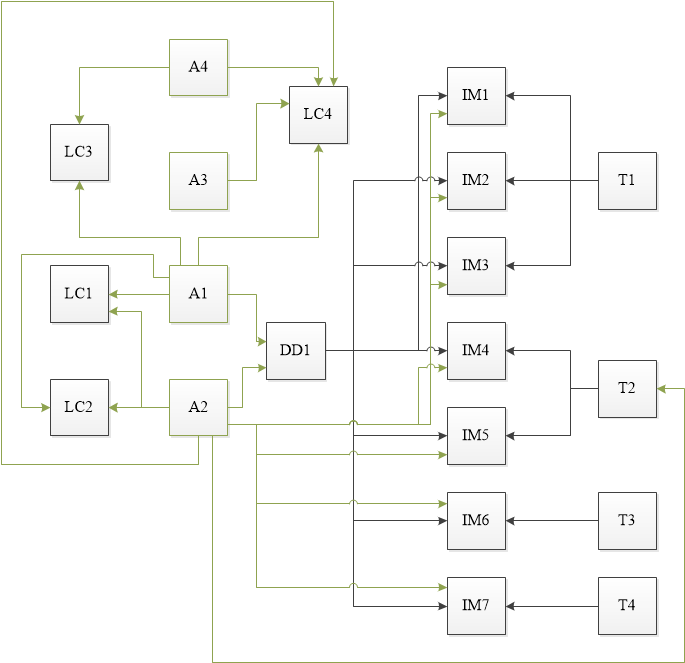
\includegraphics[width=0.96\textwidth]{figures/ATrace.png}
 		}
 		\caption{\label{Fig_ATrace} Traceability Matrix Showing the Connections 
 		Between Items of Different Sections}
 	\end{center}
 \end{figure}


 \begin{figure}[h!]
 	\begin{center}
 		%\rotatebox{-90}
 		{
 			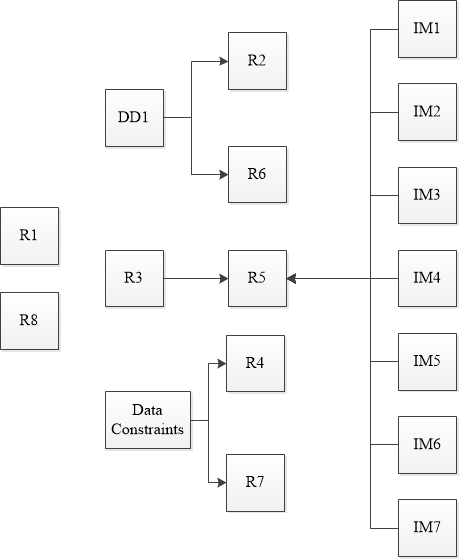
\includegraphics[width=0.65\textwidth]{figures/RTrace.png}
 		}
 		\caption{\label{Fig_RTrace} Traceability Matrix Showing the Connections 
 		Between Requirements, Instance Models, and Data Constraints}
 	\end{center}
 \end{figure}

\newpage

\bibliographystyle {plainnat}
\bibliography 
{../../ReferenceMaterial/SRS_Refs,../../ReferenceMaterial/ProblemStatement_Refs}

%\newpage
%
%\section{Appendix}
%
%\wss{Your report may require an appendix.  For instance, this is a good point 
%to
%show the values of the symbolic parameters introduced in the report.}
%
%\subsection{Symbolic Parameters}
%
%\renewcommand{\arraystretch}{1.2}
%\begin{tabular}{l l} 		
%	$\varmathbb{R}$ & Domain of real numbers\\
%\end{tabular}\\

\end{document}